\chapter{Metodologia} 
\label{chap:metodologia}

O objetivo deste trabalho é propor e investigar uma arquitetura de aprendizado profundo que unifica \textit{features} de radiômica e \textit{features} profundas. Inicialmente, é empregado diversas técnicas de aprendizado de máquina para extrair \textit{features} manuais de imagens de RM, abrangendo textura, forma, escala de cinza, etc. Posteriormente, uma rede \textit{ResNet50} pré-treinada é utilizada para extrair \textit{features} profundas que encapsulam informações semânticas de alto nível e de representação das imagens de RM. Estas \textit{features} são então fundidas em um vetor de \textit{features} unificado. Para aprimorar a acurácia e a robustez, um módulo de \textit{self-attention} foi desenvolvido. Utilizando o mecanismo de \textit{self-attention}, este módulo otimiza e pondera o vetor de \textit{features} fundidas de forma eficaz.

%---------------------------------------------------------
\section{Métodos}
\label{sec:cap4_metodos}

%---------------------------------------------------------
\subsection{ResNet}
\label{subsec:cap4_resnet}
As redes residuais, ou \textit{ResNet}, desenvolvidas por \cite{heDeepResidualLearning2015}, são arquiteturas convolucionais formada pela composição de blocos residuais, seguidos de uma camada completamente conectada. Estes blocos, ilustrados na Figura 11, empregam o que os autores chamam de \textit{skip connections}, conexões que permitem que camadas sejam puladas durante o treino, resolvendo o problema conhecido como \textit{vanishing gradient}, que afeta principalmente redes neurais profundas e impede o treinamento de progredir por conta de valores muito baixos de gradiente. A inovação trazida por este modelo permitiu a criação de redes muito mais profundas e pode possuir um número definido de camadas, portanto o uso de nomes como ResNet50 ou ResNet101 é uma prática comum para identificar a quantidade de camadas utilizadas no modelo.

%---------------------------------------------------------
\subsection{Features Radiômicas}
\label{subsec:cap4_features_radiomicas}

Foi extraído 72 \textit{features} radiômicas de fase diastólica, representada por um conjunto de fatias variando entre 6 e 18 \textit{frames}, de cada paciente usando matriz de coocorrência de níveis de cinza (GLCM) e estatísticas baseadas em histograma. Foi aplicado o filtro \textit{Laplace of Gaussian} (LoG) com cinco diferentes valores em cada parte para suavizar as imagens e realçar as bordas. Foi calculado \textit{features} GLCM como contraste, entropia, correlação, homogeneidade e energia para cada filtro LoG. Também é calculado \textit{features} de intensidade como média, variância, média dos percentis (10 e 90), desvio robusto da média absoluta, curtose e assimetria usando estatísticas de primeira ordem. Foram obtidos 78 \textit{features} radiômicas para cada paciente dentro da quantidade de fatias extraídas na fase diastólica.

%---------------------------------------------------------
\subsection{Features Profundas}
\label{subsec:cap4_features_profundas}
 
Para extrair características profundas das imagens de RM, é utilizada a arquitetura pré-treinada de um \textit{ResNet50} sem sua última camada totalmente conectada, treinada no conjunto de dados ImageNet. Estudos anteriores demonstraram que o pré-treinamento com ImageNet pode melhorar o desempenho de tarefas de classificação de imagens médicas. ResNet50 é um modelo de rede neural convolucional profunda com 50 camadas que compreende muitos blocos residuais. Cada bloco contém módulos de convolução e uma conexão de salto que transfere a informação do bloco anterior para o próximo bloco. A conexão de salto ajuda a reter a informação semântica mais básica aprendida nas camadas anteriores, que de outra forma se tornaria abstrata devido à conexão de longa cadeia. A conexão de salto também evita o desaparecimento do gradiente nas camadas mais profundas ao fornecer um caminho alternativo para a retropropagação. A informação da conexão de salto é adicionada à informação calculada em cada bloco \cite{aiSelfAttentionBasedFusion2023}. Ao todo são 2048 \textit{features} coletadas da saída deste modelo.

%---------------------------------------------------------
\subsection{Unificando as Features}
\label{subsec:cap4_unificando_features}

Um vez em posse das features radiômicas, é aplicado um F-Test tanto às 78 \textit{features} radiômicas quanto às 2048 \textit{features} profundas, reduzindo cada um dos vetores ao espaço de 64 \textit{features}. No método de fusão convencional, é simplesmente concatenado os dois vetores de \textit{features} como na Eq. \ref{eq:concat}, onde \textit{Concat} simplesmente concatena os dois vetores. Unificando ambos os vetores obtemos um vetor de 128 \textit{features} o qual passará pelo mecanismo de \textit{self-attention}.

\begin{equation}
F_{hd} = \textit{Concat}(F_h, F_d)
\label{eq:concat}
\end{equation}

%---------------------------------------------------------
\subsection{Módulo de Fusão de Self-Attention}
\label{subsec:cap4_mod_self_attention}

Neste trabalho é empregado o mecanismo de \textit{self-attention} para aprender a importância de cada \textit{feature} e capturar suas dependências de longo alcance. Como ilustrado na Figura 11111, o módulo de fusão de \textit{self-attention} é utilizado para mapear uma consulta ($Q$), chave ($K$) e valor ($V$) para um valor de \textit{attention}. Utilizamos as 128 \textit{features} concatenadas $F_{hd}$  como \textit{tokens} e projetamos cada \textit{feature} em três matrizes aprendíveis: matriz chave $K$, matriz consulta $Q$ e matriz de valor $V$ por produto escalar com as matrizes $W_{Q}$, $W_{K}$ e $W_{V}$. Logo os valores $Q$, $K$, $V$ são denotados como $W_{Q}F_{gd}$, $W_{K}F_{gd}$, $W_{V}F_{gd}$ respectivamente, onde $W_{Q}$, $W_{K}$ e $W_{V}$ representam a transformação linear para as matrizes $Q$, $K$ e $V$. O módulo de fusão baseado em \textit{self-attention} é definido como segue na Equação \ref{eq:attention}, onde $d_{k}$ é a dimensão do valor de $K$. Sem utilizar operações recorrentes ou convolucionais, o módulo de fusão de \textit{self-attention} pode modelar as dependências de longo prazo entre as características de entrada.      Este módulo calcula de forma adaptativa os pesos entre as \textit{features} com base em sua importância e relevância, capturando de forma mais abrangente as associações entre \textit{features} radiômicas e profundas. Tal processo realça a capacidade expressiva das \textit{features} fundidas e permite que o modelo foque mais precisamente nas \textit{features} mais informativas para prever \gls{CH} e reduzir a influência de características irrelevantes na previsão. Além disso, o modelo pode alocar dinamicamente \textit{attention} a diferentes amostras de imagens de \gls{RM}. Essa flexibilidade permite com que o modelo se adapte melhor à representação de \textit{features} de diferentes amostras, melhorando a precisão e a generalização da previsão.

%---------------------------------------------------------
\subsection{Função de Perda}
\label{subsec:cap4_funcao_perda}

A função de perda utilizada utilizada no modelo é a função de entropia cruzada binária, do termo  \gls{BCE}, que é calculada pela Eq. (\ref{eq:bce}) onde $\mathcal{L}_{bce}$ denota o \gls{BCE}, $N$ denota o número de imagens de \gls{RM}, $r$ denota a classe alvo de \gls{CH} e $\hat{r}$ o valor previsto de pelo modelo de \gls{CH}, 1 indica indícios de \gls{CH} e 0 sua ausência.

\begin{equation}
\mathcal{L}_{bce} = -\frac{1}{N} \sum_{i=1}^N
(r_i \ln \hat{r}_i + (1 - r_i) \ln (1 - \hat{r}_i))
\label{eq:bce}
\end{equation}

%---------------------------------------------------------
\subsection{Arquitetura Proposta}
\label{subsec:cap4_arquitetura_proposta}

O esquemático da arquitetura proposta pode ser conferida na Figura \ref{fig:fig011}. A imagens de \gls{RM} são expostas ao seletor de \textit{features} via \textit{F-test}, as \textit{features} selecionadas são concatenadas e enviados ao módulo de fusão \textit{self-attention}, por fim uma camada linear de 128 \textit{features} precede um camada linear com um único neurônio e função de ativação sigmoide para a classificação binária.

\begin{figure}[htbp]
    \centering
    \caption{Arquitetura Proposta}
    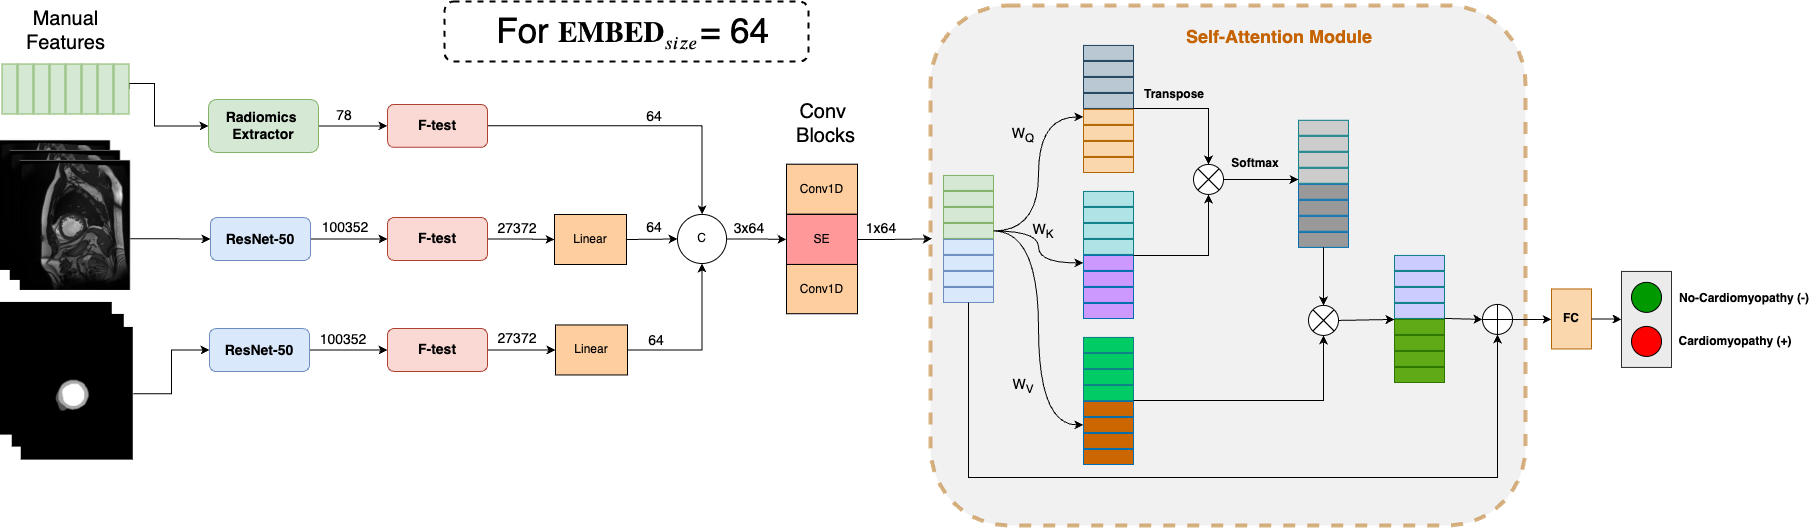
\includegraphics[width=1\textwidth]{figures/fig011.png}
    \caption*{Fonte: Autor}
    \label{fig:fig011}
\end{figure}

%---------------------------------------------------------

% \subsection{Unificando as Features}
% \label{subsec:cap4_unificando_features}

% Um vez em posse das features radiômicas, é aplicado um F-Test e reduz-se cada um dos vetores à 64 \textit{features}. Unificando ambos os vetores obtemos um vetor de \textit{features} de tamanho 128 o qual passará pelo mecanismo de \textit{attention}.

%---------------------------------------------------------
\section{Considerações Finais do Capítulo}
\label{sec:cap4_consideracoes_finais}

Como considerações finais deste capítulo, destacamos o uso de \textit{dataset} público, com dados de pacientes incluindo o conjuntos de fatias que identificam a ação de sístole e diástole do coração. É aplicado pré-processamento para onde é extraído manualmente 78 \textit{features} radiômicas, \textit{features} estas que analisam textura, níveis e variações dos tons de cinza incluindo diversas estatísticas como de primeira ordem e o \gls{GLCM}. Ainda em fase de pré-processamento é extraída as \textit{features} profundas oriundos do modelo de visão \textit{ResNet50}, com os pesos treinados no \textit{dataset} da \textit{ImageNet}. É removida a última camada linear da \textit{ResNet50} resultando ao seu final, sem a camada classificadora, 2048 \textit{features}. Em posse de ambas as features, é aplicada a técnica de \textit{F-test} para obter as 64 \textit{features} mais relevantes e, após, concatená-las obtendo um vetor de características de 128 \textit{features}. Este vetor é exposto ao módulo de fusão com \textit{self-attention}, identificando as \textit{features} mais determinantes independente de espacialidade. Ao fim o modelo entrega a classificação binária se o paciente apresenta ou não quadro de \gls{CH}. Como resultado obtido, temos um AUC de 0,74.